%
\documentclass[10pt,a4paper]{article}


\usepackage{array}
\usepackage{subfigure}
\usepackage{graphicx}
\usepackage{amssymb}
\usepackage{amsmath}
\usepackage{cite}
\usepackage{color}
\usepackage{url}
\usepackage[lined,linesnumbered,ruled,norelsize]{algorithm2e}
\usepackage{listings}
\lstset{
  language=Octave, 
  basicstyle=\footnotesize, 
  frame=single, 
  showspaces=false, 
  showstringspaces=false}




\begin{document}

\title{Experiment 8: K-Means}

\maketitle
  
\section{Description}
%
  In this exercise, you will use K-means to compress an image by reducing the number of colors it contains. To begin, download \textsf{data6.zip} and unpack its contents into your Matlab/Octave working directory.

  Photo credit: The bird photo used in this exercise belongs to Frank Wouters and is used with his permission.
  


\section{Image Representation}
%
  The data pack for this exercise contains a 538-pixel by 538-pixel TIFF image named \textsf{bird\_large.tiff}. It looks like the picture below.
  %
  \begin{figure}[htb!]
    \centering
      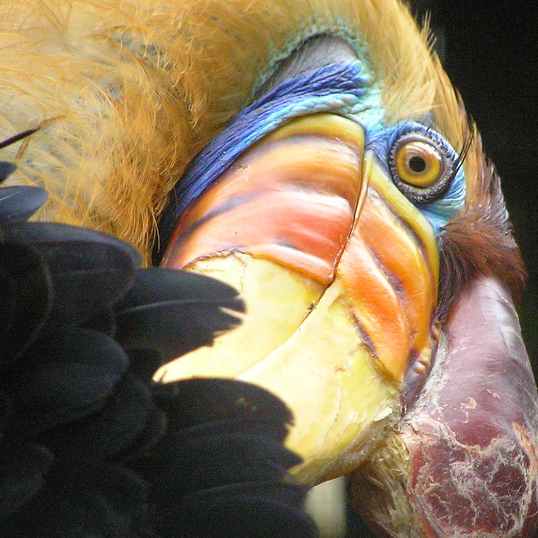
\includegraphics[width=.7\columnwidth]{bird_large}
  \end{figure}
  %
  
  %Notice that this is the same as the Gaussian kernel in the video lectures, except that term  $\frac{1}{2\sigma^2}$ in the Gaussian kernel has been replaced by $\gamma$. Once again, remember that at no point will you need to calculate $\phi(x)$ directly. In fact, $\phi(x)$ is infinite dimensional for this kernel, so storing it in memory would be impossible.

  In a straightforward 24-bit color representation of this image, each pixel is represented as three 8-bit numbers (ranging from 0 to 255) that specify red, green and blue intensity values. Our bird photo contains thousands of colors, but we'd like to reduce that number to 16. By making this reduction, it would be possible to represent the photo in a more efficient way by storing only the RGB values of the 16 colors present in the image.

  In this exercise, you will use K-means to reduce the color count to $k = 16$. That is, you will compute 16 colors as the cluster centroids and replace each pixel in the image with its nearest cluster centroid color.

  Because computing cluster centroids on a 538x538 image would be time-consuming on a desktop computer, you will instead run K-means on the 128$\times$128 image \textsf{bird\_small.tiff}.
  %
  \begin{figure}[htb!]
    \centering
      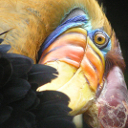
\includegraphics[width=.3\columnwidth]{bird_small}
  \end{figure}
  %
  Once you have computed the cluster centroids on the small image, you will then use the 16 colors to replace the pixels in the large image.




\section{K-means in Matlab/Octave}
%
  In Matlab/Octave, load the small image into your program with the following command:
  %
  \begin{lstlisting}
    A = double(imread('bird_small.tiff'));
  \end{lstlisting}

  This creates a three-dimensional matrix A whose first two indices identify a pixel position and whose last index represents red, green, or blue. For example, $A(50, 33, 3)$ gives you the blue intensity of the pixel at position $y = 50$, $x = 33$. (The y-position is given first, but this does not matter so much in our example because the x and y dimensions have the same size).

  Your task is to compute 16 cluster centroids from this image, with each centroid being a vector of length three that holds a set of RGB values. Here is the K-means algorithm as it applies to this problem:




  \subsection{K-Means Algorithm}
  %
  \begin{enumerate}
    \item For initialization, sample 16 colors randomly from the original small picture. These are your $k$ means  $\mu_1, \mu_2, \ldots , \mu_k$.
    \item Go through each pixel in the small image and calculate its nearest mean. 
      \begin{displaymath}
        c^{(i)} := \arg\min_{j}\left\Vert x^{(i)}-\mu_{j}\right\Vert ^{2}
      \end{displaymath}
    \item Update the values of the means based on the pixels assigned to them. 
      \begin{displaymath}
        \mu_{j}:=\frac{\sum_{i}^{m}1\{c^{(i)}=j\}x^{(i)}}{\sum_{i}^{m}1\{c^{(i)}=j\}}
      \end{displaymath}
    \item Repeat steps 2 and 3 until convergence. This should take between 30 and 100 iterations. You can either run the loop for a preset maximum number of iterations, or you can decide to terminate the loop when the locations of the means are no longer changing by a significant amount.
  \end{enumerate}


  In Step 3, you should update a mean only if there are pixels assigned to it. Otherwise, you will see a divide-by-zero error. For example, it's possible that during initialization, two of the means will be initialized to the same color (i.e. black). Depending on your implementation, all of the pixels in the photo that are closest to that color may get assigned to one of the means, leaving the other mean with no assigned pixels.




  \subsection{Reassigning Colors to The Large Image}
  %
  After K-means has converged, load the large image into your program and replace each of its pixels with the nearest of the centroid colors you found from the small image.

  When you have recalculated the large image, you can display and save it in the following way:
  %
  \begin{lstlisting}
    %Display
    imshow(uint8(round(large_image)))

    % Save image
    imwrite(uint8(round(large_image)), 'bird_kmeans.tiff');
  \end{lstlisting}
  %
  %When you are finished, compare your image to the one in the solutions.







\end{document}
